% WARNING: CE DOCUMENT NE PEUT PAS BUILD AVEC LUALATEX
% IL FAUT TROUVER UNE SOLUTION !!!

\documentclass[a4paper,landscape,twocolumn]{article}

\usepackage{préambule}
\usepackage{pstricks}

% unité de longueur pour pstricks
\psset{unit=0.4cm}


%%%%%%%%%%%%%%%%%%

\title{Activité : alignements célestes}
\date{}

%%%%%%%%%%%%%%%%%%


\begin{document}

\noindent\textbf{\huge \myuline{Activité : alignements célestes}}
\vspace{1em}

\begin{mybox}
	Les planètes et autres objets du ciel tournent à un rythme régulier dans le ciel, autour du Soleil, de la Terre, ou d’autres planètes.

	Pour les fans d’astronomie, cela peut mener à des phénomènes passionnants, comme les éclipses, ou les alignements de planètes.

	Mais comment savoir à quel moment un tel évènement va arriver ?
\end{mybox}
\begin{question}
	On commence par étudier le mouvement, plus simple, de 2 satellites artificiels de la Terre :
	\begin{itemize}
		\item Le satellite Astérix, qui fait le tour de la Terre en 3 jours.
		\item Le satellite Ohsumi, qui fait le tour de la Terre en 5 jours
	\end{itemize}

	\begin{figure}[h!]
		\captionsetup{labelformat=empty}
		\begin{floatrow}
			\ffigbox{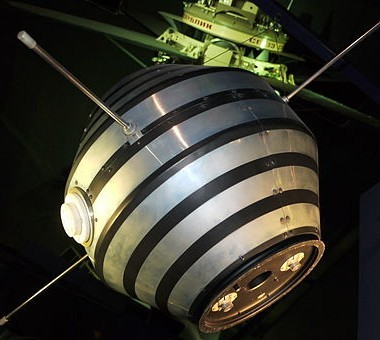
\includegraphics[width=0.3\linewidth]{Satellite_Asterix.JPG}}
			{\caption{Satellite Astérix}}

			\ffigbox{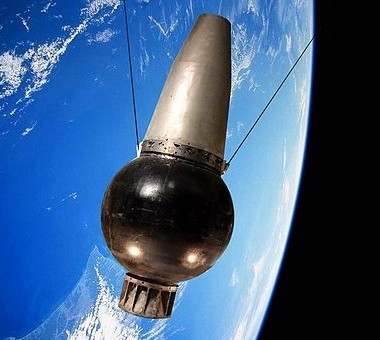
\includegraphics[width=0.3\linewidth]{Satellite_Ohsumi.jpg}}
			{\caption{Satellite Ohsumi}}
		\end{floatrow}
	\end{figure}
	\begin{itemize}
		\item[\textbf{a.}] Au 1\textsuperscript{er} septembre, les satellites étaient alignés au-dessus de Lyon. Quand seront-ils à nouveau alignés au-dessus de Lyon ?
		\item[\textbf{b.}] Tous les combien de jours ces satellites vont-ils s'aligner au-dessus de Lyon ?

		      Le nombre trouvé est un .............. de 3 et de 5.
	\end{itemize}
\end{question}

\newpage

\begin{question}
	On s'intéresse cette fois aux satellites  	Aryabhata et Azur, qui sont passés au-dessus de Lyon le 1\textsuperscript{er} octobre :
	\begin{itemize}
		\item Aryabhata fait le tour de la Terre en 6 jours.
		\item Azur fait le tour de la Terre en 4 jours.
	\end{itemize}

	\begin{figure}[h!]
		\captionsetup{labelformat=empty}
		\begin{floatrow}
			\ffigbox{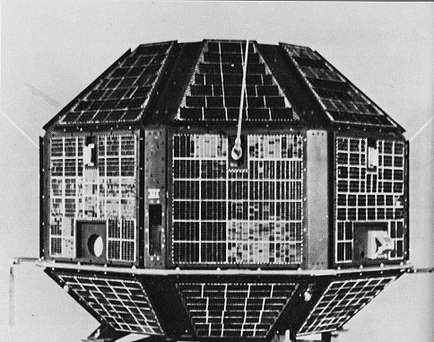
\includegraphics[width=0.3\linewidth]{Satellite_Aryabhata.jpg}}
			{\caption{Satellite Aryabhata}}

			\ffigbox{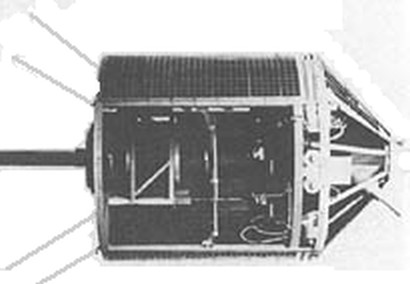
\includegraphics[width=0.3\linewidth]{Satellite_Azur.jpg}}
			{\caption{Satellite Azur}}
		\end{floatrow}
	\end{figure}

	\begin{itemize}
		\item[\textbf{a.}] Au vu de la question précédente, tous les combien de temps ces deux satellites s'alignent-ils ?
		\item[\textbf{b.}] Les 2 droites ci-dessous représentent le calendrier d'octobre (seuls les jours impairs sont notés pour ne pas prendre trop de place).

		      Pour chaque satellite, marquer ses passages au-dessus de Lyon par une croix :

		      \begin{pspicture}(1,1)
			    %   \psdots[dotstyle=+,dotscale=3,dotangle=45](0,0)
			    %   \psaxes[
				%       yAxis=false,
				%       linecolor=blue,
				%       Ox={1},
				%       Dx=2,
				%       xsubticks=2,
			    %   ]{->}(0,0)(0,0)(32,0)
		      \end{pspicture}

		    %   \vspace{1cm}
		    %   Aryabhata

		    %   \begin{pspicture}(1,1)
			%       \psdots[dotstyle=+,dotscale=3,dotangle=45](0,0)
			%       \psaxes[
			% 	      yAxis=false,
			% 	      linecolor=blue,
			% 	      Ox={1},
			% 	      Dx=2,
			% 	      xsubticks=2,
			%       ]{->}(0,0)(0,0)(32,0)
		    %   \end{pspicture}

		      \vspace{1cm}
		      Azur
		      \vspace{0.7cm}
		\item[\textbf{c.}] Pouvez-vous modifier votre réponse à la question a. ?
	\end{itemize}
\end{question}

\newpage

\begin{question}
	Toutes les planètes tournent autour du soleil.

	Le 13 juin 2021, les planètes Mercure et Vénus étaient alignées avec le soleil.

	\begin{itemize}
		\item[\textbf{a.}] A quelle date seront-elles dans l'exact même position ?
		\item[\textbf{b.}] Le dernier alignement de Mercure, Vénus et la Terre était le 18 septembre 1934. Quand aura lieu le prochain alignement similaire ?
	\end{itemize}
\end{question}

\begin{center}
	\begin{TAB}(r,0cm,0.6cm){|c|c|}{|c|c|c|c|c|c|c|c|c|}
		\textbf{Planète} & \textbf{Temps pour tourner autour du soleil} \\
		% 2*2*2*11
		Mercure & 88 jours \\
		% 2*2*5*11
		Vénus & 220 jours \\
		% 5*73
		Terre & 365 jours \\
		% 3*229
		Mars & 687 jours \\
		% 2*2*3*19*19
		Jupiter & 4 332 jours \\
		Saturne & 10 754 jours \\
		Uranus & 30 698 jours \\
		Neptune & 60 217 jours \\
	\end{TAB}

	\vspace{0.2cm}
	Périodes de rotation des planètes du système solaire.
\end{center}

\newpage

\begin{greybox}[frametitle={Point historique et scientifique}]
	\begin{itemize}
		\item Les satellites Astérix, Ohsumi, Aryabhata et Azur sont les premiers satellites envoyés par la France, le Japon, l'Inde et l'Allemagne respectivement.
		\item Le temps qu'ils mettent à faire le tour de la Terre a été inventé pour l'exercice. Aryabhata et Azur ne sont même plus dans le ciel !
		\item Pour l'exercice, la période de rotation de Vénus a été légèrement changée. En vérité, Vénus met 225 jours pour faire le tour du soleil.
	\end{itemize}
\end{greybox}

\begin{greybox}[frametitle={Pour jouer avec le système solaire}]
	\url{https://www.planete-astronomie.eu/systeme-solaire-interactif-3d.html}
\end{greybox}

\end{document}